\documentclass[11pt,letterpaper]{article}
\usepackage[utf8]{inputenc}

%----- Configuración del estilo del documento------%
\usepackage[table]{xcolor}
\usepackage{epsfig,graphicx}
\usepackage[left=2cm,right=2cm,top=1.8cm,bottom=2.3cm]{geometry}
\usepackage{fancyhdr}
\usepackage{lastpage}
\pagestyle{fancy}
\fancyhf{}
\rfoot{\textit{Página \thepage \hspace{1pt} de \pageref{LastPage}}}


%------ Paquetes matemáticos básicos --------%
\usepackage{amsmath}
\usepackage{amssymb}
\usepackage{amsthm}

%------ Texto aleatorio ----- %

\usepackage{lipsum}
\usepackage{enumitem}


\begin{document}

%------ Encabezado -------- %

\begin{center}
    \begin{minipage}{3cm}
    	\begin{center}
    		\includegraphics[height=3.4cm]{./imagenes/logo_unam.png}
    	\end{center}
    \end{minipage}\hfill
    \begin{minipage}{10cm}
    	\begin{center}
    	\textbf{\large Universidad Nacional Autónoma de México}\\[0.1cm]
        \textbf{Facultad de Ciencias}\\[0.1cm]
        \textbf{Matemáticas para las Ciencias Aplicadas 2$|$ Grupo 7056}\\[0.1cm]
        \textbf{Tarea 1 }\\[0.1cm]
        Cisneros Álvarez Danjiro\\[0.1cm]
        Rodríguez López Luis Fernando\\[0.1cm]
        Tenorio Reyes Ihebel Luro\\[0.1cm]
        25/11/2024
    	\end{center}
    \end{minipage}\hfill
    \begin{minipage}{3cm}
    	\begin{center}
    		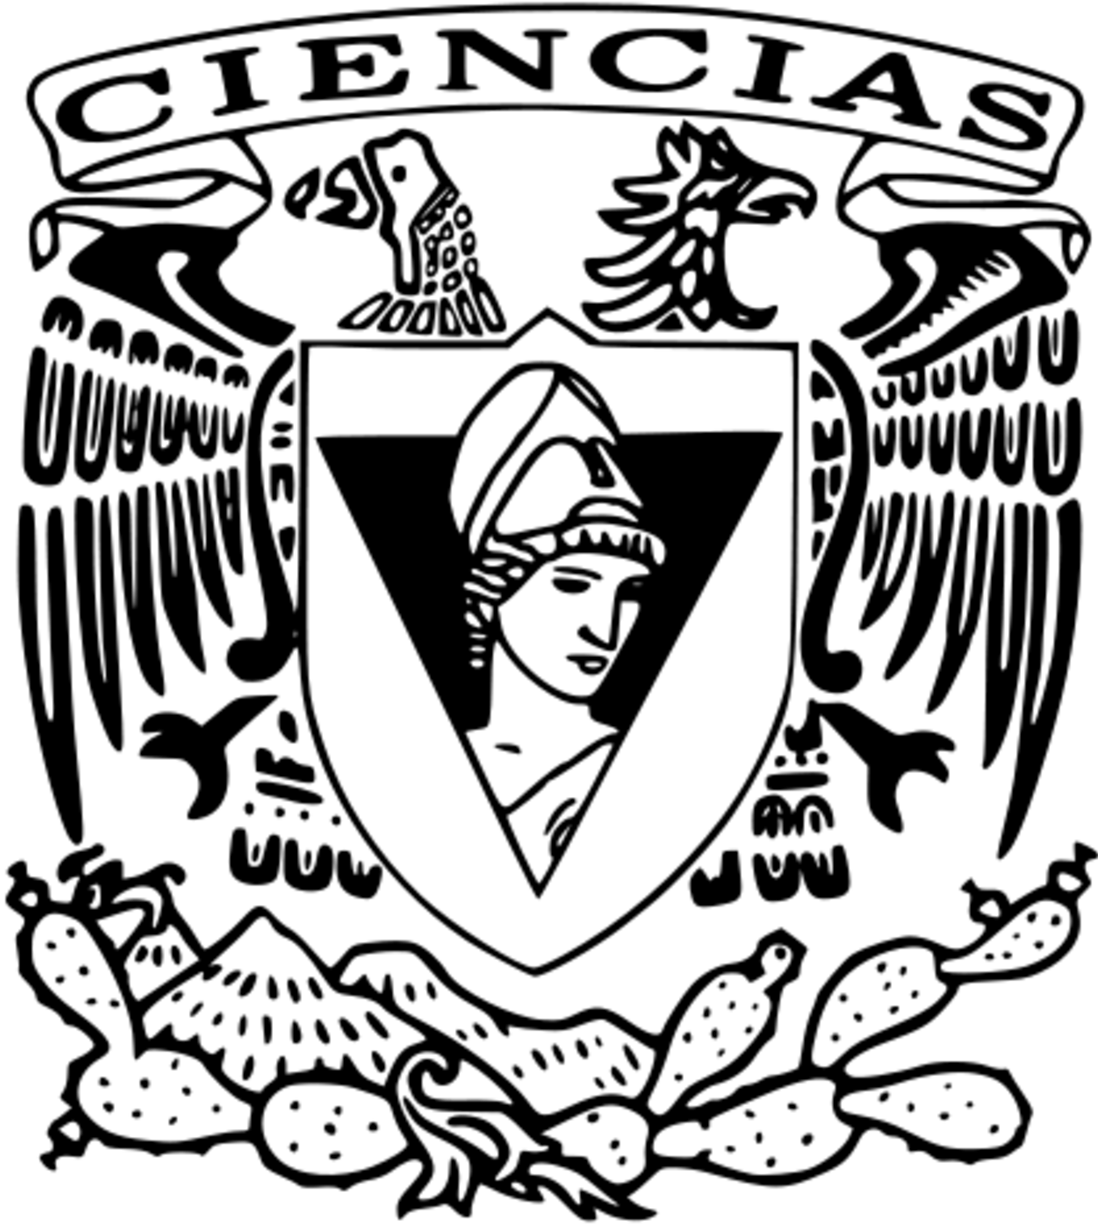
\includegraphics[height=3.4cm]{./imagenes/Logo_FC.png}
    	\end{center}
    \end{minipage}
\end{center}

\rule{17cm}{0.1mm}

%------ Fin de encabezado -------- %

%\section*{1ra Parte}

\subparagraph{Ejercicios: Sección 11.2 Anton-Bivens-Davis (pp. 782-784).}

% ---- 01. Ejercicio 52 DANJIRO ---- %
\section{Ejercicio 52, Sección 11.2}

% ---- 02. Ejercicio 56 LUIS ---- %
\section{Ejercicio 56, Sección 11.2}

% ---- 03. Ejercicio 58 IHEBEL ---- %
\section{Ejercicio 58, Sección 11.2}


\subparagraph{Ejercicios: Sección 11.3 Anton-Bivens-Davis (pp. 792-794).}

% ---- 04. Ejercicio 19 LUIS ---- %
\section{Ejercicio 19, Sección 11.3}

% ---- 05. Ejercicio 34 IHEBEL ---- %
\section{Ejercicio 34, Sección 11.3}

% ---- 06. Ejercicio 35 DANJIRO ---- %
\section{Ejercicio 35, Sección 11.3}

% ---- 07. Ejercicio 36 LUIS ---- %
\section{Ejercicio 36, Sección 11.3}



\subparagraph{Ejercicios: Sección 11.4 Anton-Bivens-Davis (pp. 803-805).}

% ---- 08. Ejercicio 40 IHEBEL ---- %
\section{Ejercicio 40, Sección 11.4}

% ---- 09. Ejercicio 41 DANJIRO ---- %
\section{Ejercicio 41, Sección 11.4}

% ---- 10. Ejercicio 49 POR SORTEAR ---- %
\section{Ejercicio 49, Sección 11.4}

\end{document}